\documentclass[tikz,border=10pt]{standalone}
\begin{document}
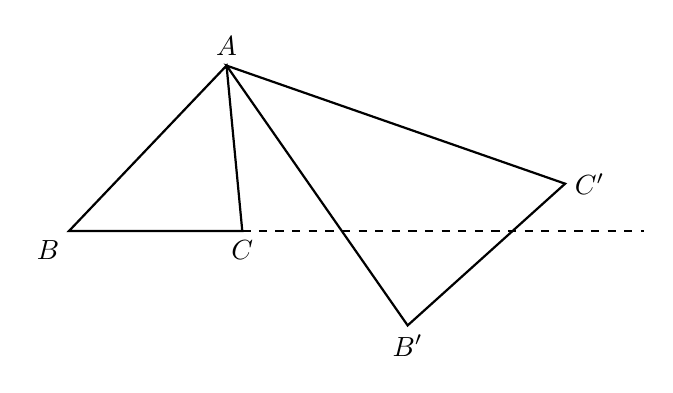
\begin{tikzpicture}
  \coordinate (A) at (2,3.6);
  \coordinate (B) at (0,1.5);
  \coordinate (C) at (2.2,1.5);
  \coordinate (Bp) at (4.3,0.3);
  \coordinate (Cp) at (6.3,2.1);

  \draw[thick] (B) -- (A) -- (C) -- cycle;
  \draw[thick] (A) -- (Bp) -- (Cp) -- cycle;
  \draw[thick,dashed] (C) -- (7.3,1.5);

  \node[above] at (A) {$A$};
  \node[below left] at (B) {$B$};
  \node[below] at (C) {$C$};
  \node[below] at (Bp) {$B'$};
  \node[right] at (Cp) {$C'$};
\end{tikzpicture}
\end{document}
